%-----------------------------------LICENSE------------------------------------%
%   This file is part of tikz_figures.                                         %
%                                                                              %
%   tikz_figures is free software: you can redistribute it and/or              %
%   modify it it under the terms of the GNU General Public License as          %
%   published by the Free Software Foundation, either version 3 of the         %
%   License, or (at your option) any later version.                            %
%                                                                              %
%   tikz_figures is distributed in the hope that it will be useful,            %
%   but WITHOUT ANY WARRANTY; without even the implied warranty of             %
%   MERCHANTABILITY or FITNESS FOR A PARTICULAR PURPOSE.  See the              %
%   GNU General Public License for more details.                               %
%                                                                              %
%   You should have received a copy of the GNU General Public License along    %
%   with tikz_figures.  If not, see <https://www.gnu.org/licenses/>.           %
%------------------------------------------------------------------------------%

% Use the standalone class for displaying the tikz image on a small PDF.
\documentclass[crop, tikz]{standalone}

% Import the tikz package to use for the drawing.
\usepackage{tikz}

% tikz packages used.
\usetikzlibrary{arrows.meta, angles, quotes}

% Begin the document.
\begin{document}

    % Begin the drawing.
    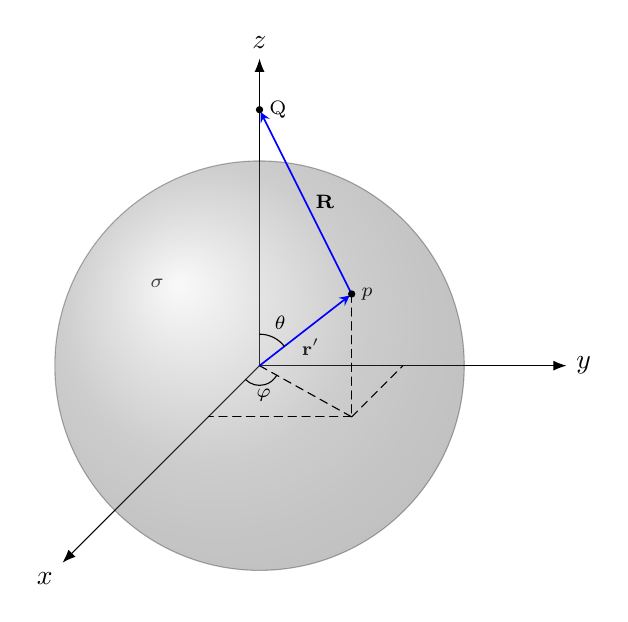
\begin{tikzpicture}[%
        line width = 0.4pt,
        line cap = round,
        > = Latex,
        scale = 1.3
    ]

        % Positions for the points in the drawing.
        \coordinate (z) at (0.0, 1.0, 0.0);
        \coordinate (x) at (0.0, 0.0, 1.0);
        \coordinate (o) at (0.0, 0.0, 0.0);
        \coordinate (p1) at (0.9, -0.5, 0.0);
        \coordinate (p2) at (1.4, 0.0, 0.0);
        \coordinate (p3) at (-0.5, -0.5, 0.0);
        \coordinate (Q) at (0.0, 2.5, 0.0);
        \coordinate (p) at (0.9, 0.7, 0.0);

        % Add all of the labels.
        \node at (Q) [right] {\scriptsize{Q}};
        \node at (p) [right] {\scriptsize{$p$}};
        \node at (-1, 0.8, 0.0) {\scriptsize{$\sigma$}};
        \node at (0.5, 0.18, 0.0) {\scriptsize{$\mathbf{r}'$}};

        % Draw the coordinate axes.
        \draw[->] (0.0, 0.0, 0.0) to (3.0, 0.0, 0.0) node[right] {$y$};
        \draw[->] (0.0, 0.0, 0.0) to (0.0, 3.0, 0.0) node[above] {$z$};
        \draw[->] (0.0, 0.0, 0.0) to (0.0, 0.0, 5.0) node[below left] {$x$};

        % Use ball-color to mimic a 3D sphere being drawn.
        \draw[ball color = gray, opacity = 0.3] (0.0, 0.0, 0.0) circle (2.0);

        % Dashed lines for the projections on to the xy plane.
        \begin{scope}[densely dashed]
            \draw (o) to (p1);
            \draw (p) to (p1);
            \draw (p1) to (p2);
            \draw (p1) to (p3);
        \end{scope}

        % Position vector for P, and relative position vector PQ.
        \begin{scope}[%
            ->,
            > = stealth,
            draw = blue,
            semithick,
            shorten > = 0.33mm
        ]
            \draw (o) to (p);
            \draw (p) to node[right] {\scriptsize{$\mathbf{R}$}}(Q);
        \end{scope}

        % Label the points P and Q.
        \draw[fill = black] (Q) circle (0.3mm);
        \draw[fill = black] (p) circle (0.3mm);

        % Draw the angle made with respect to the z axis.
        \pic[%
            draw = black,
            "\scriptsize{$\theta$}",
            angle eccentricity = 1.5,
            angle radius = 0.4cm
        ] {angle = p--o--z};

        % And lastly, draw the azimuthal angle made in the xy plane.
        \pic[%
            draw = black,
            "\scriptsize{$\varphi$}",
            angle eccentricity = 1.5,
            angle radius = 0.25cm
        ] {angle = x--o--p1};
    \end{tikzpicture}
\end{document}
